\documentclass{article}
\usepackage{graphicx, amsmath, float, siunitx, hyperref, mathtools} % Required for inserting images
\usepackage[ngerman]{babel}
\usepackage{biblatex, csquotes}
\addbibresource{refs.bib}
\usepackage[
  locale=DE,
  separate-uncertainty=true,
  per-mode=symbol
]{siunitx}

\DeclareSIUnit\gauss{G}

\newcommand{\abb}{{\color{red}\textbf{{ABB.XYZ}}} }
\newcommand{\Oszi}{Oszilloskop }

\usepackage{caption}
\usepackage{subcaption}

\usepackage{csvsimple}
\usepackage{comment}
\usepackage{booktabs}

\title{Praktikum V - Kern- und Teilchenphysik\\Versuch 521 - $\gamma$-Spektroskopie mit Szintillations- und Halbleiterdetektoren}

\author{Tom Chelius und Alican Özcagi}
\date{24. April 2025}

\begin{document}

\maketitle
\tableofcontents

\newpage
\section{Einleitung}

\section{Theorie}

\section{Voraufgabe}
Es sollte für ein gegebenes Spektrum ein Skript geschrieben werden, womit es möglich ist die Spektrallinien zu analysieren. Hierbei wurde eine Anpassungsfunktion der Form
\begin{equation}
    H + A \cdot \exp{\frac{-(x_i-\mu_i )^2}{2 \sigma_i^2}}
\end{equation}
verwendet und an die jeweiligen gaußförmigen Linien angepasst, die Anpassungsparameter sind in Tabelle \ref{tab:voraufgabe} zu sehen und die Anpassungen an den Graphen in \ref{}


\begin{table}
    \centering
    \begin{tabular}{|c|c|c|c|c|c|c|} \hline
      Peaknummer & A & $\Delta A$ & $\mu$ & $\Delta \mu$ & $\sigma$ & $\Delta \sigma$\\ \hline \hline
        1 & 457.36 & 19.99 & 330.18 & 0.12 & 35.11 & 0.22 \\ \hline
        2 & 47.66 & 106.46 & 599.44 & 76.85 & 67.21 & 396.49\\ \hline
        3 & 65.64 & 97.34 &  796.09 & 1408.61 & 93.56 & 867.42\\ \hline
        4 & 250.00 & 891.00 & 922.10 & 3.80 & 50.11 & 6.99\\ \hline
        5 & 37.95 & 5.39 & 3234.32 & 171.14 & 248.58 & 305.13\\ \hline
        6 & 87.79 & 5.10 & 3917.53 & 21.81 & 152.34 & 27.84\\ \hline
    \end{tabular}
    \caption{Anpassung an spectrum.txt aus der Voraufgabe}
    \label{tab:voraufgabe}
\end{table}

\begin{figure}
    \centering
    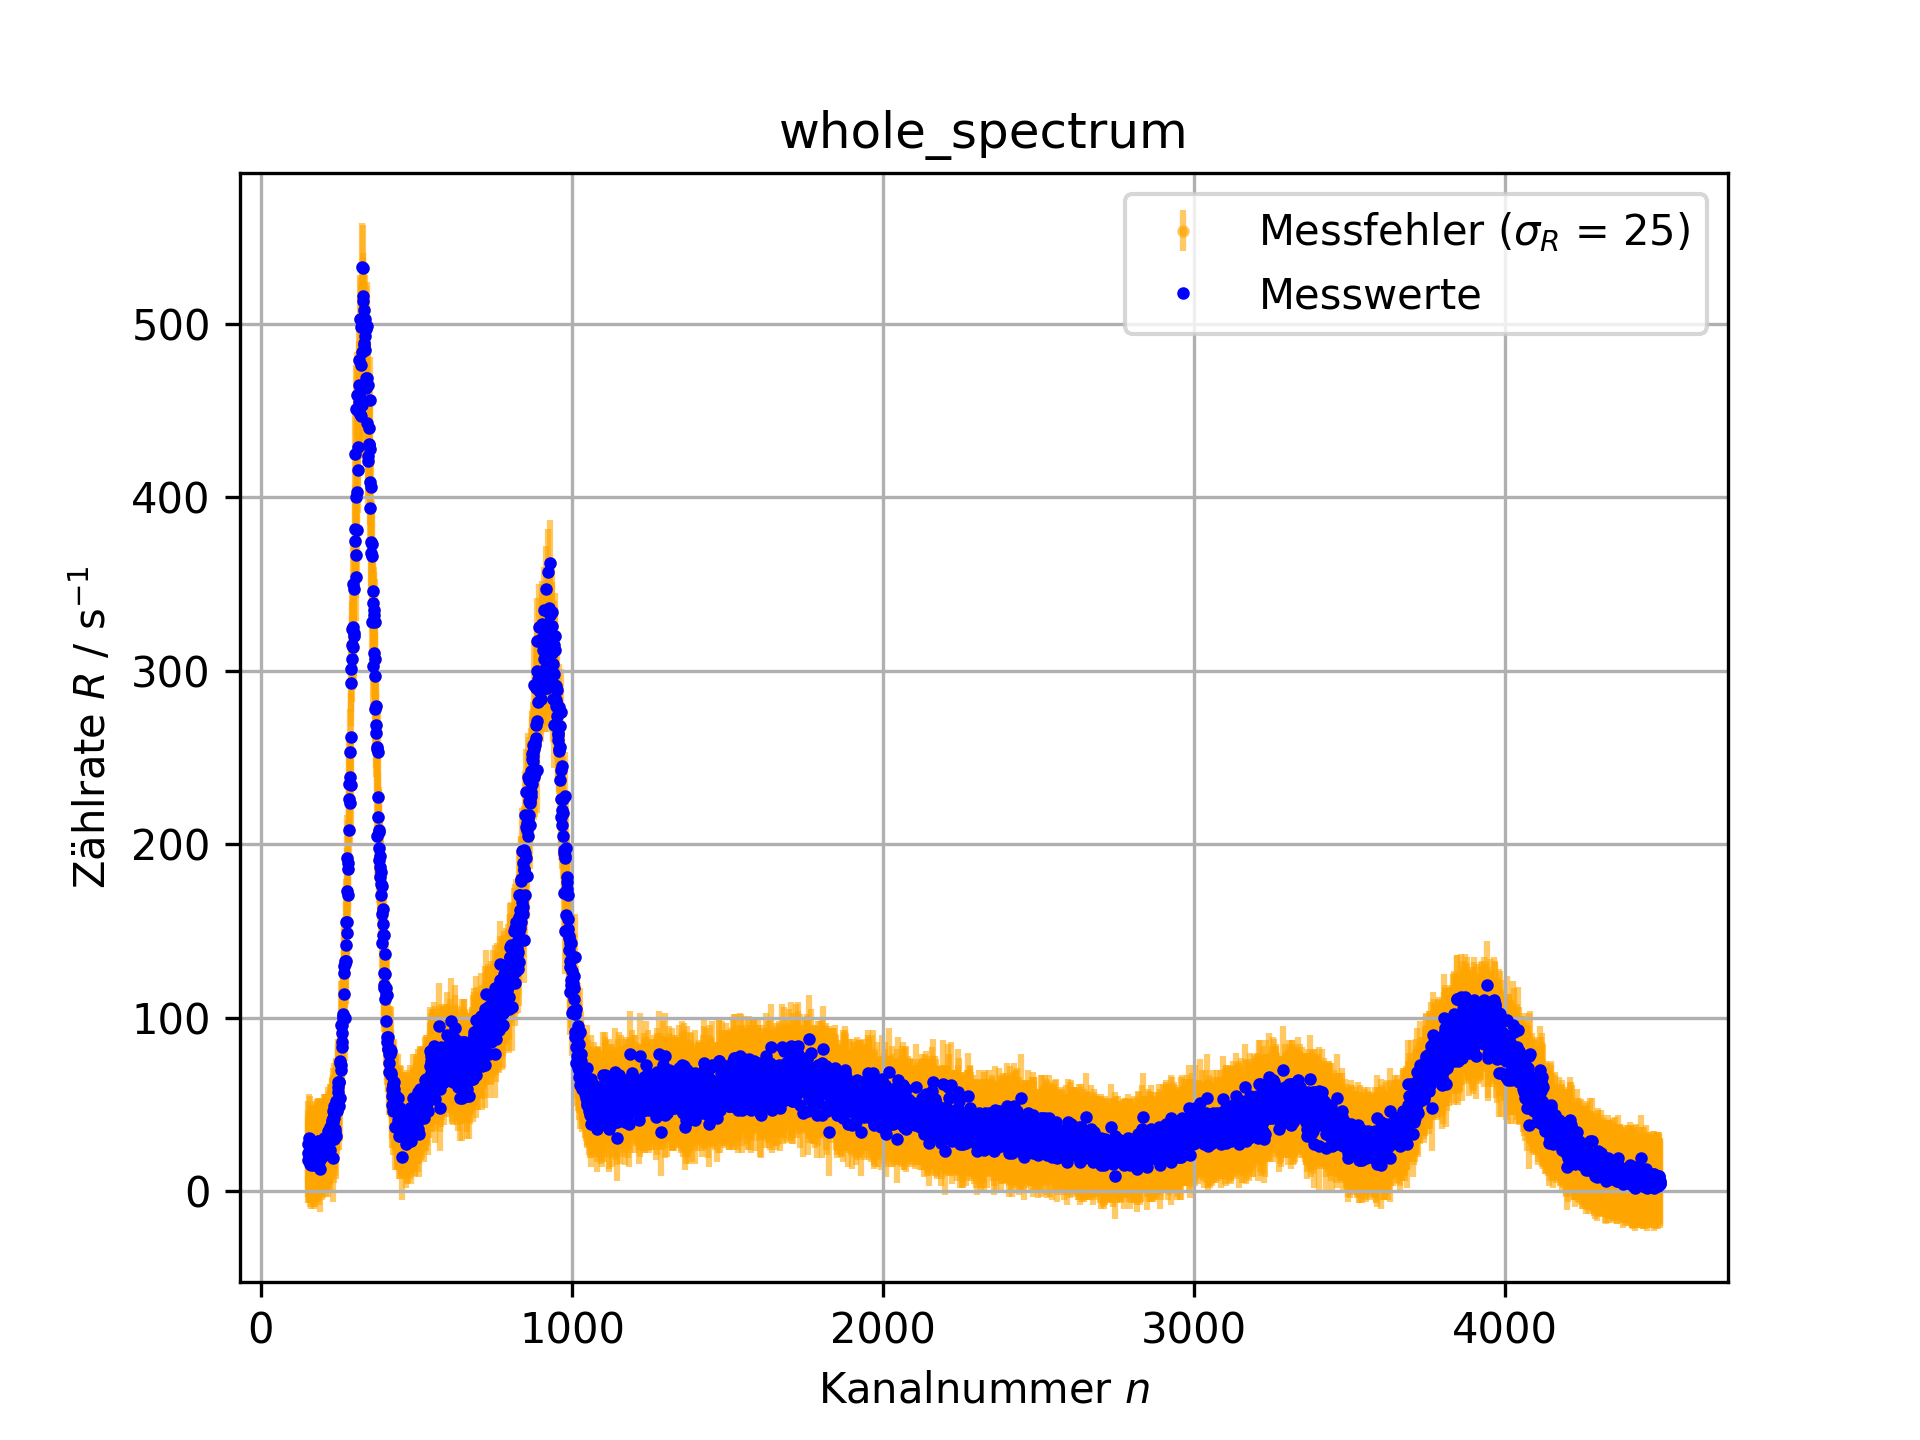
\includegraphics[width=1\linewidth]{/figures/whole_spectrum.png}
    \caption{Anpassungsfunktion}
    \label{fig:voraufgabeFig}
\end{figure}

\newpage
\printbibliography[heading=bibintoc]

\end{document}